In this chapter, we'll begin

\todo{introduction}

\section{Intersection Theory}

Throughout this chapter, we'll adopt the convention that $X$ is an ambient $n$-dimensional oriented manifold with boundary, and $M$ and $N$ are closed manifolds. We'll assume that all closed submanifolds of $X$ and smooth maps from a closed manifold to $X$ avoid the boundary.

\begin{definition}\label{def:transverse-intersection-basic}
	Two submanifolds $M,N\subset X$ are said to \defn{intersect tranversally} or to be \defn{transverse} if for all points $p\in M\cap N$ we have $\T_p M\oplus \T_p N = \T_p X$.
\end{definition}

\begin{figure}[ht]
	\centering
	\import{graphics/temp-diagrams/}{transverse-intersection.pdf_tex}
	\medskip
	\caption{Examples and non-examples of transverse intersections in $\R^3$.}\label{fig:transverse-intersection}
\end{figure}

If we lose the assumption that the spaces we're considering aren't smoothly embedded submanifolds of the ambient space, but rather images of a smooth map then this definition can be slightly generalized.

\begin{definition}\label{def:transverse-intersection}
	If $f : N \to X$ and $g : M \to X$ are smooth maps, we say that $f$ and $g$ are \defn{transverse} if for all $p\in N$ and $q\in M$ with $f(p)=g(q)=x\in X$, we have
	\[
		\T_x X = df_p(\T_p N) \oplus dg_q(\T_q M).
	\]
\end{definition}

\begin{remark}
When $f$ and $g$ are embeddings, this recovers \cref{def:transverse-intersection-basic}.
\end{remark}

While it's easy to come up with examples of manifolds which aren't transverse, there is a mathematical sense in which ``almost all'' submanifolds intersect transversally.

\begin{theorem}
	Let $C^\infty(N,X)$ be the space of all maps from a compact manifold $N$ to some ambient manifold $X$. If we fix a submanifold $M\subset X$, then the subset
	\[
		C^\infty_{\mathrm{tv.}\,M}(N,X)=\{ f : N \to X \mid f\textrm{ is transverse to } M\}\subset C^\infty(N,X)
	\]
	of maps transverse to $M$ is a dense subset of $C^\infty(N,X)$.
\end{theorem}

\begin{proof}
	See the proof of Theorems~6.35 in \cite{lee2012smooth}.
\end{proof}

In simpler terms, this density of transverse maps implies that transversality is a \defn{stable}[stable property] and \defn{generic}[generic property] property. Stability in this context means that it is resilient to perturbations (if a map is transverse to $M$, perturbing it slightly will keep it transverse to $M$), and generality means that if a map is not transverse to $M$, we can perturb it slightly to make it transverse.
What this means for us is that without much loss of generality, we can assume that all manifolds and smooth maps intersect transversally.

\begin{figure}[ht]
	\centering
	\import{graphics/temp-diagrams/}{perturbing-intersection-transverse.pdf_tex}
	\medskip
	\caption{Perturbing a manifold embedding to get a transverse intersection.}\label{fig:perturbing-intersections-transverse}
\end{figure}

The observant reader might remark that there isn't a way of measuring distances between maps in $C^\infty(N,X)$, this would require more than just the topological data we have access to. We do however have a notion of homotopy, so whenever refer to stability, generality, and perturbation, we use the following formal definition.

\begin{definition}
	Suppose we have a property $\mathcal{P}$ of functions between topological spaces.
	\begin{enumerate}
		\item The property $\mathcal{P}$ is said to be \defn{stable}[stable property] if for every function $f : X \to Y$ satisfying $\mathcal{P}$ and homotopy $H : X\times[0,1]\to Y$ with $H(x,0) = f(x)$, there exists an $\varepsilon>0$ such that for all $s\in [0,\varepsilon)$, the function $H(x,s)$ also satisfies $\mathcal{P}$.
		\item The property $\mathcal{P}$ is said to be \defn{generic}[generic property] if for every function $f : X \to Y$ \emph{not} satisfying $\mathcal{P}$ and arbitrary $\varepsilon>0$, there is a homotopy $H : X\times [0,\varepsilon] \to Y$ with $H(x,0)=f(x)$ such that the function $H(x,\varepsilon)$ satisfies $\mathcal{P}$.
	\end{enumerate}
\end{definition}

\subsection{The Oriented Intersection Number}

One of the fundamental properties concerning transverse maps is that they behave well when taking intersections, or more generally when taking preimages. This forms the backbone of the intersection theory of manifolds.

\begin{theorem}[Preimage Theorem]\label{thm:preimage}
	If $f : N \to X$ is a smooth map transverse to a submanifold $M\subset X$ then $S=f^{-1}(M)\subset N$ is a submanifold with the same codimension in $N$ as $M$ in $X$.
\end{theorem}
\begin{proof}
	See the proof of Theorem~6.30 in \cite{lee2012smooth}.
\end{proof}

\begin{remark}\label{rmk:symmetric-preimage-theorem}
	We can get a symmetric version of this theorem as a straightforward corollary. If we have two transverse maps $f : N\to X$ and $g : M\to X$, then the map $f\times g : N\times M \to X\times X$ is transverse to the diagonal submanifold $\Delta\subset X\times X$. \cref{thm:preimage} will then imply that 
	\[
		(f\times g)^{-1}(\Delta) \subset M\times N
	\]
	is a submanifold. When $g$ is an embedding, $(f\times g)^{-1}(\Delta)$ can be projected down onto $M$ to get the preimage $f^{-1}(M)$.
\end{remark}

If the manifolds involved in \cref{thm:preimage} are orientable, this preimage $S$ admits a canonical orientation by the following procedure. First of all, recall that for any embedded manifold $M\subset X$ there is an exact sequence of vector bundles by quotienting
\begin{equation}\label{eq:oriented-intersection-number-1}
	\begin{tikzcd}
		0 & {\T M} & {\T X} & {\T X/M} & 0
		\arrow[from=1-1, to=1-2]
		\arrow[from=1-2, to=1-3]
		\arrow[from=1-3, to=1-4]
		\arrow[from=1-4, to=1-5]
	\end{tikzcd}
\end{equation}
where $\T X/M$ is the normal bundle of $M\subset X$. Using the orientations of $X$ and $M$, we can use this exact sequence to get an orientation of the normal bundle $\T X/M$. At every point $p\in S$ of the preimage, the differential map $df$ connects the sequence \cref{eq:oriented-intersection-number-1} to the normal bundle sequence for the embedding $S\subset N$.
\begin{equation}\label{eq:oriented-intersection-number-2}
	\begin{tikzcd}
		0 & {\T_pS} & {\T_p N} & {\T_p N/S} & 0 \\
		0 & {\T_{f(p)}M} & {\T_{f(p)}X} & {\T_{f(p)}X/M} & 0
		\arrow[from=1-1, to=1-2]
		\arrow[from=1-2, to=1-3]
		\arrow["{df_p}", from=1-2, to=2-2]
		\arrow[from=1-3, to=1-4]
		\arrow["{df_p}", from=1-3, to=2-3]
		\arrow[from=1-4, to=1-5]
		\arrow["{df_p}", from=1-4, to=2-4]
		\arrow[from=2-1, to=2-2]
		\arrow[from=2-2, to=2-3]
		\arrow[from=2-3, to=2-4]
		\arrow[from=2-4, to=2-5]
	\end{tikzcd}
\end{equation}
In this diagram \cref{eq:oriented-intersection-number-2}, the rightmost vertical map is an isomorphism by the transversality of $f$ and $M$. This means that we can pullback the orientation on $\T_{f(p)} X/M$ to $\T_p N/S$. Since $\T_p N$ is oriented, the usual ``2-out-of-3'' rule applied to the top row of \cref{eq:oriented-intersection-number-2} gives an orientation of $\T_p S$. See \cref{fig:preimage-orientation} for an example of this orienting procedure.

\begin{figure}[ht]
	\centering
	\import{graphics/temp-diagrams/}{preimage-orientation.pdf_tex}
	\medskip
	\caption{Orienting a preimage (assuming a clockwise orientation on $X$ and $N$).}\label{fig:preimage-orientation}
\end{figure}

When $M$ and $N$ have complementary dimensions, the preimage $S=f^{-1}(N)\subset M$ is a compact oriented $0$-dimensional manifold. For each point $p\in S$, we have $\T_p S=0$ so the map $\T_p N\to \T_p N/S$ in \cref{eq:oriented-intersection-number-2} is an isomorphism. The orientation of $N$ gives an orientation of $\T_p N$, and the preimage orientation procedure gives us an orientation of $\T_p N/S$. Now we can define:

\begin{definition}
The \defn{local (oriented) intersection number}[oriented intersection number (local)] of $f$ and $M$ at $p\in S$ is
\[
	\#_p^X(f, M) = \begin{cases}
		+1 & \T_p N/S \textrm{ has the same orientation as } \T_p N,     \\
		-1 & \T_p N/S \textrm{ has the opposite orientation to } \T_p N.
	\end{cases}
\]
\end{definition}
Summing over all of the local intersection numbers gives a global quantity.
\begin{definition}
	The \defn{(oriented) intersection number}[oriented intersection number] of a smooth map $f : N \to X$ intersecting a submanifold $M\subset X$ transversally is
	\[
		\#^X(f, M) = \sum_{p\in S} \#_p^X(f, M) \in \Z.
	\]
\end{definition}

\begin{remark}\label{rmk:symmetric-intersection-number}
	For a more symmetric version of this definition when two smooth maps $f : N \to X$ and $g : M \to X$ intersect transversally, we could take inspiration from \cref{rmk:symmetric-preimage-theorem} and define the oriented intersection number of the smooth maps $f$ and $g$ as
	\[
		\#^X(f,g) = \#^{X\times X}(f\times g, \Delta).
	\]
	This symmetric intersection number is graded commutative in the dimensions of $M$ and $N$, i.e.
	\begin{equation}\label{eq:intersection-number-graded-commutative}
		\#^X(f,g) = (-1)^{\dim M\cdot \dim N} \#^X(g,f)
	\end{equation}
\end{remark}

Just as the property of transversality is stable -- resilient to homotopic perturbations -- so too is the oriented intersection number. This follows as a corollary to a more general theorem.

\begin{theorem}
	If $W$ is a compact oriented manifold with boundary, and $H : W \to X$ is a smooth map, then $\#^X(\partial H, M)=0$. Here, we use the notation $\partial H : \partial W \to X$ to refer to the restriction of $H$ to the boundary of $W$.
\end{theorem}

\begin{corollary}
	If $H : [0,1]\times N \to X$ is a smooth homotopy, then $\#^X(H_0, M) = \#^X(H_1, M)$.
\end{corollary}

Applying the construction of the symmetric oriented intersection number gives a map
\begin{equation}\label{eq:oriented-intersection-number-homotopy}
	\lkxfunc{\#^X}{[N,X]\times [M,X]}{\Z}{f,g}{\#^X(f,g)}
\end{equation}
This is a geometric precursor to the intersection form of a manifold, a central object of study in geometric topology. 

Finally, we'll state a useful result in computer self-intersection numbers -- a way to compute the intersection number of a submanifold with itself.

\begin{theorem}\label{thm:euler-number-self-intersection}
	If $M$ is a closed $m$-dimensional submanifold of a $2m$-dimensional submanifold $X$ then we have
	\[
		\#^X(M, M) = \chi(\T X/M)
	\]
	where $\chi(\T X/M)$ is the Euler number of the normal bundle of $M$.
\end{theorem}
\begin{proof}
	\todo{todo}
\end{proof}

\begin{corollary}\label{thm:euler-number-self-intersection-corollary}
	The Euler number $\chi(\xi)$ of an oriented real vector bundle $\xi : E \to B$ over a compact oriented manifold can be expressed as the intersection number
	\[
		\#^E(z,z) = \chi(\xi)
	\]
	where $z : B \to E$ is the zero section.
\end{corollary}

\subsection{Homology Classes and Submanifolds}

Let $f : N\subset X$ be a smooth map from a compact oriented $p$-dimensional manifold $N$ to $X$. The data of an orientation on a closed manifold gives a fundamental class $[N]\in \H_p(N)$ which can be pushed forward along the map $f : N \hookrightarrow X$ to give us a homology class $f_* [N]\in \H_p(X)$. This is the homology class associated to a smooth map $N\to X$.
This correspondence behaves nicely with respect to perturbations, and thus as we will later see, with transversality.
Suppose $H : N\times [0,1] \to X$ is a homotopy with $H(x,0)=f(x)$ which perturbs the map $f$. For any $\varepsilon>0$, the map $f_\varepsilon : N \to X$ given by $f_\varepsilon(x)=H(x,\varepsilon)$ is homotopic to $f$ and hence induces the same map on homology $\H_p(N)\to \H_p(X)$. The homology class associated to a map $f : N \to X$ thus solely depends on the homotopy type of $f$ so we get a map
\[
	\lkxfunc{}{[N,X]}{\H_p(X).}
\]
Letting $N=S^p$, we can see that this is a generalization of the Hurewicz homomorphism which links homotopy groups to homology groups via a map $\pi_p(X) \to \H_p(X)$.
As with the Hurewicz homomorphism, this correspondence is generally not surjective or injective. If a space is $k$-connected for $k\geq 1$ then we have a Hurewicz isomorphism $\pi_{k+1}(X) \to \H_{k+1}(X)$ which means that every homology cycle in $\H_{k+1}(X)$ can at least be represented by a smooth map of a sphere $S^{k+1}$ into $X$. This smooth map might have ``double-points'', i.e. when multiple points of the sphere map to the same point in the image and prevent the smooth map from being an embedding.

\begin{example}
	In the punctured plane $X=\R^2\setminus \{0\}$ with homology $\H_1(X)\cong \Z$, the only homology cycles which can be represented by embedded submanifolds are $0,\pm 1$, by a circle not containing the origin and circles of both orientations surrounding the origin respectively. A smooth map representing a cycle of higher degree would necessarily have a double-point as in \cref{fig:double-point}.
\end{example}

\begin{figure}[ht]
	\centering
	\import{graphics/temp-diagrams/}{double-point.pdf_tex}
	\caption{A double-point in a smooth map representing $\pm 2\in \H_1(\R^2\setminus\{0\})$.}\label{fig:double-point}
\end{figure}

That being said, many specially constructed manifolds we will consider in this chapter will at least have a basis by embedded submanifolds, and every homology class will admit a representation by a smooth map. For a classical account of some issues that can arise when representing homology classes by smooth maps, see Chapter II of Ren\'e Thom's seminal paper \cite{thom1954}.

\begin{remark}
	In some special cases, homology classes can \emph{always} be represented by embedded submanifolds. For instance, if $X$ is a $4$-manifold, there are isomorphisms
	\[
		\H^2(X; \Z) \cong [X, K(\Z,2)] \cong [X, \CP^\infty] \cong [X,\CP^2],
	\]
	where the first is the representability of singular cohomology by the Eilenberg-Maclane spectrum, the second identifies $\CP^\infty$ as a $K(\Z,2)$ space, and the third uses the cellular approximation theorem. Any cohomology cycle $\omega\in \H^2(X)$ can be represented by a smooth function $f : X \to \CP^2$. If we choose this function to be transverse to $\CP^1\subset \CP^2$, then $f^{-1}(\CP^1)$ is an embedded $2$-dimensional submanifold of $X$ which corresponds to a Poincar\'e dual class to $\omega$. When $X$ is a compact manifold, Poincar\'e duality tells us that all $2$-dimensional homology cycles can be represented by embedded submanifolds in this way. This is one reason why $4$-manifolds (especially simply-connected $4$-manifolds) are such wonderful geometric objects of study!
\end{remark}

Now let's see if our previously defined notion of an oriented intersection number transfers over as an operation on homology classes. Recall that by the Poincar\'e-Lefschetz duality for compact manifolds with boundary, there is an isomorphism
\[
	\lkxfunc{}{\H^{n-p}(X,\partial X)}{\H_p(X)}{\omega}{\omega\frown [X,\partial X]}
\]
given an orientation class $[X,\partial X]\in \H_n(X, \partial X)$. Under this duality, there is a geometric interpretation of the cup product on cohomology cycles as the oriented intersection number for submanifolds representing the dual homology cycles (when such a representation is possible). We can define this homology intersection pairing $\tnsv$ as the top map in the commutative square
\begin{equation}\label{eq:homology-intersection}
	\begin{tikzcd}
		{\H_p(X)\otimes \H_q(X)} & {\H_{n-p-q}(X)} \\
		{\H^{n-p}(X, \partial X)\otimes \H^{n-q}(X,\partial X)} & {\H^{2n-p-q}(X,\partial X)}
		\arrow["\tnsv", from=1-1, to=1-2]
		\arrow[tail reversed, from=1-1, to=2-1]
		\arrow[tail reversed, from=1-2, to=2-2]
		\arrow["\smile", from=2-1, to=2-2]
	\end{tikzcd}
\end{equation}
where the vertical maps are the Poincar\'e-Lefschetz isomorphism. Finally, we have our link between the algebra of (co)homology and the differential topology of intersections.

\begin{theorem}
	Suppose $M,N\subset X$ are transverse oriented submanifolds. Then we have
	\[\iota_*[M]\tnsv \iota_*[N] = \#_X(M,N)\]
\end{theorem}
\begin{proof}
	\todo{todo}
\end{proof}

As suggested by the map in \cref{eq:oriented-intersection-number-homotopy}, we now have an entirely algebraic object which encapsulates the geometry of intersections on a manifold. 

\begin{definition}
	Let $X$ be an oriented $2m$-dimensional manifold, possibly with boundary. The \defn{intersection form} on middle dimensional homology is the bilinear form
	\[
		\lkxfunc{Q_X}{\H_m(X)_{\mathrm{free}}\otimes \H_m(X)_{\mathrm{free}}}{\Z}{\alpha\otimes \beta}{\alpha\tnsv \beta}
	\]
	where we identify $\H_0(X)\cong \Z$ and $\H_m(X)_{\mathrm{free}}$ denotes the free component of $\H_m(X)$ -- i.e. the quotient by torsion elements.
\end{definition}

Since $\smile$ is graded-commutative, by \cref{eq:homology-intersection} so is $\tnsv$. Of course, we would expect the graded-commutativity as a generalization of \cref{eq:intersection-number-graded-commutative}. This implies:
\begin{proposition}
	If $m$ is even then $Q_X$ is a symmetric bilinear form and if $m$ is odd then $Q_X$ is a skew-symmetric bilinear form.
\end{proposition}

Examples of intersection forms are plentiful.
\begin{example}
	The intersection form for the 4-dimensional torus $T^4=S^2\times S^2$ can be represented by the hyperbolic matrix
	\[
		Q_{T^4} = \begin{pmatrix}0 & 1 \\ 1 & 0\end{pmatrix}.
	\]
	where we use the basis for $\H_2(T^4)$ given by the embedded submanifolds $S^2\times \{p\}$ and $\{p\}\times S^2$ for some $p\in S^2$. If we call these homology classes $\alpha$ and $\beta$, it's clear that we have $\alpha \tnsv \beta = 1$ since they intersect transversally at the singular point $(p,p)$ and we normalize orientations so that $\alpha\tnsv \beta$ is positive. It also follows that $\alpha\tnsv \alpha = 0$ since the submanifolds $S^2\times \{p\}$ and $S^2\times \{q\}$ have empty intersection for $p\neq q$ and both represent the homology cycle $\alpha$.
\end{example}

\begin{example}
	The intersection form for any even-dimensional complex projective plane $\CP^{2m}$ is given by $Q_{\CP^{2m}}=(1)$.
\end{example}

\begin{example}
	In algebraic geometry, the quartic K3 surface
	\[
		\textrm{K3} = \left\{ [z_0 : z_1 : z_2 : z_3]\in \CP^3 \mid z_0^4 + z_1^4+z_2^4 + z_3^4=0\right\}
	\]
	has the intersection form $Q_{\textrm{K3}} = -2\cdot \E_8 \oplus 3\cdot H$ where $H$ is the $2\times 2$ hyperbolic matrix and $\E_8$ an $8\times 8$ matrix defined in \cref{defn:E8-matrix}.
\end{example}

\subsection{Connected Sum}

\todo{write this}

\begin{figure}[ht]
	\centering
	\import{graphics/temp-diagrams/}{connected-sum.pdf_tex}
	\caption{Construction of the connected sum.}\label{fig:connected-sum}
\end{figure}

\begin{proposition}\label{prop:connected-sum-intersection-form}
	If $X$ and $Y$ are $2m$-dimensional manifolds, then we have
	\[Q_{X\+Y} = Q_X\oplus Q_Y\]
\end{proposition}
\begin{proof}
	\todo{todo}
\end{proof}

\subsection{Highly-Connected Manifolds}

The simplest class of manifolds for which the intersection form is an interesting invariant are known as highly-connected manifolds. Highly-connected manifolds contain the minimal amount of (co)homological data for which to define an intersection form, and this makes them an attractive target for classification and construction.

\begin{definition}
	A compact $2m$-dimensional manifold $X$ is said to be \defn{highly-connected} if it is $(m-1)$-connected. Consequently, $X$ has non-trivial (co)homology only in the middle dimension $\H_m(X)$ and in the usual extremal dimensions $\H_0(X)$ and $\H_{2m}(X)$.
\end{definition}

\begin{remark}
	In fact, it was the attempted classification of highly-connected manifolds in dimension $8$ which led to the first discovery of an exotic sphere by Milnor in 1956, see \cite{milnor2000exotic} for a historical account of the discvery by the man himself.
\end{remark}

\section{Plumbing}

Suppose we wanted to construct a $2m$-dimensional manifold with a given intersection form -- specified by a bilinear form $Q$ on the unit lattice $\Z^\ell$ with basis vectors $e_1,\ldots, e_\ell$. Let's call this hypothetical construction $W^{2m}$.

The simplest possible case is when the lattice is $1$-dimensional, with intersection form
\[
	Q = \begin{pmatrix} Q_{11}\end{pmatrix}
\]
determined by the single integer $Q_{11}=Q(e_1,e_1)\in \Z$.
The resulting $2m$-manifold $W$ should have middle dimensional homology $\H_m(W)$ free of rank $1$, generated by a cycle $\alpha$ which has self-intersection number $\alpha\tnsv \alpha = Q_{11}$. To construct such a manifold, let's start with a $m$-dimensional sphere $S^m$. This will be the submanifold representing the generating cycle $\alpha\in \H_m(W)$. To get a $2m$-dimensional manifold, we ``thicken'' the sphere by choosing a rank $m$ disk bundle $\xi : E \to S^m$ with Euler number $Q_{11}$ (if such a bundle exists). Note that this is equivalent to choosing a vector bundle, since we can move freely between vector and disk bundles by an associated bundle construction. We can now define $W$ as the total space $E$ of the disk bundle. This will be the base case for plumbing constructions.
\begin{figure}[ht]
	\centering
	\import{graphics/temp-diagrams/}{thickening-sphere.pdf_tex}
	\caption{Two different ``thickenings'' of $S^1$ by $D^1$ bundles.}\label{fig:thickening-sphere}
\end{figure}

Although plumbing non-orientable bundles is certainly possible and interesting in its own right, to keep the resulting manifolds orientable we'll require orientable bundles $\xi$ (this rules out the M\"obius bundle thickening in \cref{fig:thickening-sphere}). With this requirement, $W$ gets a manifold orientation from the orientation of the bundle.
Since disks are contractible, there is a deformation retraction $W\simeq S^m$, and this implies that the middle dimensional homology $\H_m(X)$ is generated by $\iota_*[S^m]$. By \cref{thm:euler-number-self-intersection-corollary}, the self intersection number of $\iota_*[S^m]$ is exactly the Euler number $\chi(\xi)$ which we set to be $Q_{11}$ by our choice of bundle $\xi$.

Vector bundles with a given Euler number don't always exist over an $m$-sphere. For instance, if $m$ is odd, then the Euler number of any bundle over $S^m$ is zero and so $Q_{11}$ must be zero in this case. This isn't a failure of the construction but rather reflects that $Q$ is skew-symmetric when $m$ is odd and so must have zeroes along the diagonal. When $m$ is even however, there are plenty of bundles which have a non-zero Euler number. For instance, the tangent bundle $\T S^m$ has Euler number $2$. This lets us construct a $4k$-manifold with boundary that has intersection form $Q = (2)$.

\subsection{Vector Bundles Over Spheres}

This is a good time for a brief interlude on vector bundles over spheres.
Vector bundles over a sphere can be classified by the clutching construction. Suppose $\xi : E \to S^m$ is a vector bundle. We can decompose the sphere $S^m$ into hemispheres $S^m=D_+^m\cup D_-^m$, and these disks intersect at the equator $D_+^m\cap D_-^m=S^{m-1}\subset S^m$ -- a sphere one dimension lower. The bundle $\xi$ can be trivialized on the hemispheres since they are contractible, and we denote these trivializations
\[
	\lkxfunc{\varphi_+}{E|_{D^m_+}}{D^m_+\times \R^m}
	\quad\textrm{and}\quad
	\lkxfunc{\varphi_-}{E|_{D^m_-}}{D_-^m \times \R^m.}\]
The trivializations must come with transition functions on their intersection (we might have to expand the intersection a bit so that it is open). The transition function is a diffeomorphism $\psi$ in the commutative diagram
\[\begin{tikzcd}
		{S^{m-1}\times \R^m} && {S^{m-1}\times \R^m} \\
		& {E|_{S^{m-1}}}
		\arrow["\psi", from=1-1, to=1-3]
		\arrow["{\varphi_+|_{S^{m-1}}}", from=2-2, to=1-1]
		\arrow["{\varphi_-|_{S^{m-1}}}"', from=2-2, to=1-3]
	\end{tikzcd}\]
which is constant on the first factor, and linear in the second factor. For each point $p\in S^{m-1}$, the diffeomorphism $\psi$ thus gives a linear function $\tau_p : \R^m \to \R^m$. These linear maps are the ``change of coordinate'' transformations between the fibers on the boundaries of $D_+^m$ and $D_-^m$ (see \cref{fig:clutching-construction}).
\begin{figure}[ht]
	\centering
	\import{graphics/temp-diagrams/}{clutching-construction.pdf_tex}
	\caption{Getting a map $\tau : S^{m-1}\to \GL_m$ from a vector bundle over $S^{m}$.}\label{fig:clutching-construction}
\end{figure}

Altogether, this family of linear transformations is indexed by the equator $S^{m-1}$, and this gives us a smooth map $\tau : S^{m-1}\to \GL_m$. It follows that the homotopy type of $\tau$ is only dependent on the isomorphism type of the bundle $\xi$ since any vector bundle isomorphism can be shown to induce a homotopy of smooth maps. In order words, we have a map
\[
	\lkxfunc{}{\op{Vect}_m(S^m)}{\pi_{m-1}(\GL_m).}
\]
sending a vector bundle $\xi$ to the its associated homotopy class $\tau\in \pi_{m-1}(\GL_m)$.

The construction works in the opposite direction as well. Whenever we have a homotopy class $\tau\in \pi_{m-1}(\GL_m)$, we can form a bundle $\xi_\tau : E_\tau \to S^{m}$ by letting
\[
	E_\tau = (D_+^m\times D^m)\cup_T (D_-^{m}\times D^m),
\]
where $T(x,y)=(x,\tau(x)y)$ is the glueing map.

\todo{write this}

A similar argument holds when we restrict to oriented bundles, i.e. vector bundles with structure group $\SO_m$.

\begin{theorem}
	The clutching construction gives bijections
	\[
		\begin{aligned}
			\lkxfunc{}{\pi_{m-1}(\O_m)}{\op{Vect}_m(S^m)} \\
			\lkxfunc{}{\pi_{m-1}(\SO_m)}{\op{Vect}_m^+(S^m)}
		\end{aligned}
	\]
	between homotopy groups of the orthogonal groups and isomorphism classes of vector bundles.
\end{theorem}
\begin{proof}
	\todo{prove}
\end{proof}

Under this correspondence the Euler number of a vector bundle can be considered as a group homomorphism
\[
	\lkxfunc{e}{\pi_{m-1}(\SO_m)}{\Z}{\tau}{e(\xi_\tau)}
\]
\begin{theorem}\label{thm:euler-number-of-vector-bundle-over-sphere}
	Let $p : \SO_{2m} \to \SO_{2m}/\SO_{2m-1}= S^{2m-1}$ be the projection map of the special orthogonal group to the sphere. Then the following diagram commutes,
	\[\begin{tikzcd}
			{\pi_{2m-1}(\SO_{2m})} & \Z \\
			{\pi_{2m-1}(S^{2m-1})}
			\arrow["e", from=1-1, to=1-2]
			\arrow["{p_*}"', from=1-1, to=2-1]
			\arrow[from=2-1, to=1-2]
		\end{tikzcd}\]
	where $\pi_{2m-1}(S^{2m-1})\to \Z$ is the degree isomorphism.
\end{theorem}
\begin{proof}
	\todo{prove}
\end{proof}

\begin{corollary}
	The image of $e : \pi_{2m-1}(\SO_{2m})\to\Z$ is $2\Z$.
\end{corollary}
\begin{proof}
	\todo{prove}
\end{proof}

\begin{remark}
	The clutching construction is a special case of a more general classification of principal $G$-bundles. Generally, if $G$ is a Lie group there is a natural isomorphism of contravariant functors
	\[
		[-, \Bclass G] \lkxto \Bun_G(-)
	\]
	where $[-, \Bclass G]$ is the set of homotopy classes of maps to a space $\Bclass G$ and $\Bun_G(-)$ is the set of isomorphism classes of principal $G$-bundles over a given space.
	The space $\Bclass G$ is known as the \defn{classifying space}\footnote{The classifying space is rarely a manifold, and is usually an infinite dimensional CW complex.} of $G$ and this space comes equipped with a \defn{universal bundle} $\zeta : \Eclass G \to \Bclass G$. With this universal bundle, the natural isomorphism is easy to describe. Under the appropriate topological restrictions, a map $\tau : X \to \Bclass G$ gives us a pullback bundle $\tau^*\zeta$ over $X$. This is a principal $G$-bundle over $X$ which is entirely determined by the homotopy type of the \defn{classifying map} $\tau$.

	In some sense, the universal bundle $\zeta$ is the ``most twisted $G$-bundle''. Pullbacks of bundles generally ``dilute'' the twistedness of a bundle -- for instance, the splitting principle allows any complex vector bundle to be pulled back to a direct sum of complex line bundles. It would stand to reason that every bundle is the pullback of a more twisted bundle, and the limit of this process is the universal bundle $\zeta$ over the classifying space. See Chapter IV of \cite{botttu1982differential} for a wonderful exposition on the topic.

	It can be shown that (under suitable topological restrictions) there is a homotopy equivalence $\Omega \Bclass G \simeq G$ where $\Omega$ denotes the loop space operator in homotopy theory. Indeed from a homotopy theory perspective, the classifying space is a ``delooping'' of the group $G$. For spheres, the loop space suspension adjunction gives us natural isomorphisms
	\[
		\begin{aligned}
			\Bun_{G}(S^m) & \cong [S^m, \Bclass G]            \\
			              & \cong [\Sigma S^{m-1}, \Bclass G] \\
			              & \cong [S^{m-1}, \Omega\Bclass G]  \\
			              & \cong [S^{m-1}, G]
			\cong \pi_{m-1}(G).
		\end{aligned}
	\]
	This is a generalized way of understanding the clutching construction.
\end{remark}

\subsection{Milnor Manifolds}

The first constructions of exotic spheres in \cite{milnor1956manifolds} were defined as the boundary of an $8$-manifold formed by taking the total space of various disk bundles over $S^4$.

\todo{finish}

\begin{definition}
	\todo{Milnor manifold}
\end{definition}

\subsection{Plumbing Multiple Bundles}

Let's now consider the case of a $2$-dimensional lattice, and try to construct a manifold with intersection form $Q$ given by the $2\times 2$ integer matrix:
\[
	Q = \begin{pmatrix} Q_{11} & Q_{12} \\ Q_{21} & Q_{22}\end{pmatrix}.
\]
This matrix should be symmetric when $m$ is even and skew-symmetric when $m$ is odd. To begin constructing a manifold, we want $\H_m(W)$ to be free of rank $2$, generated by cycles $\alpha$ and $\beta$ with intersection numbers specified by the matrix $Q$. The simplest case is when $|Q_{12}|=|Q_{21}|=0$, i.e. the intersection forms is represented by a diagonal matrix and splits as a direct sum $Q=Q_1\oplus Q_2$. In this case, by \cref{prop:connected-sum-intersection-form}, we can define
\[
	P(Q_1\oplus Q_2) = P(Q_1)\+ P(Q_2).
\]
In fact, this construction lets us realize any diagonal matrix as the intersection form of a manifold, assuming all entries along the diagonal are the Euler numbers of some oriented bundle (even if $m$ is even and zero if $m$ is odd).

The next simplest case is when $|Q_{12}|=|Q_{21}|=1$. In this case, we'd want $\H_m(W)$ to be free of rank $2$, generated by cycles $\alpha$ and $\beta$ which intersect only once. The natural thing to do would be to start with a wedge of two $m$-spheres $S^m_1\vee S^m_2$. This should be the homotopy type of the constructed manifold $W$. Next, we need to ``thicken'' this space into a $2m$-manifold by rank $m$ disk bundles $\xi_i : D(E_i) \to S^m_i$ for $i\in\{1,2\}$. However, the total spaces of these bundles still need to be glued together so as to form a manifold. This glueing can be done in a ``criss-cross'' manner. If $S^m_1$ and $S^m_2$ are wedged together at points $x_1$ and $x_2$, we begin by choosing disks $D_i^m\subset S^m_i$ which are neighborhoods of these points. The bundles $\xi_i$ then admit local trivializations, so we get neighborhoods $D_i^m\times D^m_i \subset D(E_i)$ of the points $x_i$ in the total space of the bundle. Finally, we choose diffeomorphisms $g : D_1^m \to D_2^m$ and $h : D_1^m \to D_2^m$ which either both preserve orientations or reverse them. 

\begin{definition}\label{def:plumbing}
The \defn{plumbing} of $D(E_1)$ and $D(E_2)$ at the points $x_1$ and $x_2$ is the quotient space $E_1\square E_2 =D(E_1)\cup_f D(E_2)$ where $f$ is the map
\[
		\lkxfunc{f}{D_1^m\times D_1^m}{D_2^m\times D_2^m}{(x,y)}{(h(y), g(x)).}
\]
\end{definition}

Note that away from the neighborhoods $D_1^m\subset S^m_1$ and $D_2^m\subset S^m_2$, the plumbed manifold still looks like the total space of a disk bundle. This allows us to plumb together multiple bundles, or plumb together two bundles at multiple points by choosing distinct disk neighborhoods for each point.

\begin{figure}[ht]
	\centering
	\import{graphics/temp-diagrams/}{plumbing-two-circles-smoothed.pdf_tex}
	\caption{A plumbing of two trivial circle bundles with smoothed corners.}\label{fig:plumbing-two-circles}
\end{figure}

\begin{remark}\label{rmk:smoothing-corners}
	The plumbing has an a priori smooth structure everywhere except at the ``corners'' which arise from the boundaries $\partial D_1^m\times \partial D_1^m \cong \partial D_2^m\times \partial D_2^m$ in $P$. To smooth these out, \todo{finish}
\end{remark}

Now let's study the intersection theory of the plumbed manifold. It's clear that the submanifolds $S_1^m$ and $S_2^m$ intersect transversally at a single point.

\begin{proposition}
	If $x$ is the intersection point of $S_1^m$ and $S_2^m$, then we have
	\[
		\#^{E_1\square E_2}_{x}(S_1^m, S_2^m) = \begin{cases}
		+1 & h \textrm{ and }g\textrm{ preserve orientations},\\
		-1 & h \textrm{ and }g\textrm{ reverse orientations}.\\
	\end{cases}
	\]
\end{proposition}
\begin{proof}
	\todo{cite}
\end{proof}

As a corollary, if we plumb together two bundles at $m$ points with a positive orientation (let's call this manifold $E_1\square^m E_2$), then the intersection number is $\#^{E_1\square^m E_2}(S^m_1, S^m_2)=m$. The same thing with $m$ points and a negative orientation gives the intersection number $\#^{E_1\square^{-m} E_2}(S^m_1,S^m_2)=-m$. We thus have a way to construct a $4k$-manifold $W^{4k}$ and $(4k+2)$-manifold $W^{4k+2}$ with intersection forms
\[
	Q_{W^{4k}} = \begin{pmatrix} 2e_1 & m \\ m & 2e_2\end{pmatrix}
	\quad\textrm{and}\quad
	Q_{W^{4k+2}} = \begin{pmatrix} 0 & m \\ -m & 0\end{pmatrix}
\]
for any $e_1, e_2,m\in \Z$. This approach generalizes to lattices of higher dimensions, and we arrive at the first main theorem regarding plumbing.

\begin{theorem}[Plumbing Theorem]
	Suppose $Q$ is a bilinear form over an $\ell$-dimensional lattice $\Lambda$ given by an $\ell\times \ell$ integer matrix which is symmetric if $m$ is even and skew-symmetric when $m$ is odd. When $m$ is even, we also require the matrix to have even entries along the diagonal. Then there exists a $2m$-dimensional manifold $P(Q)$ with isomorphism $\H_{m}(P(Q))\cong \Lambda$ under which the intersection form of $P(Q)$ is exactly the bilinear form $Q$.
\end{theorem}

\begin{proof}

\begin{lemma}
	For each integer $q\geq 1$, there is a homotopy equivalence
	\[
		S^m\vee_q S^m \simeq S^m\vee S^m \vee \bigvee_{q-1} S^1,
	\]
	where $S^m\vee_q S^m$ denotes the wedge sum of two $m$-spheres at $q$ points.
\end{lemma}

\begin{proof}
\end{proof}

\end{proof}

Let's now 

\subsection{Plumbing Along a Tree}

\begin{definition}
	A \defn{tree} $T$ is a finite connected contractible $1$-dimensional simplicial complex, i.e. a finite connected graph with no cycles. An \defn{weighted tree}[tree (weighted)] with weights in a set $S$ is a pair $(T,w)$ consisting of a tree $T$ and a map $w : \op{Vert}(T) \to S$ assigning a \defn{weight} $w(v)\in S$ to each vertex $v$ of the tree.
\end{definition}

\begin{figure}[ht]\label{fig:negative-definite-trees}
	\centering
	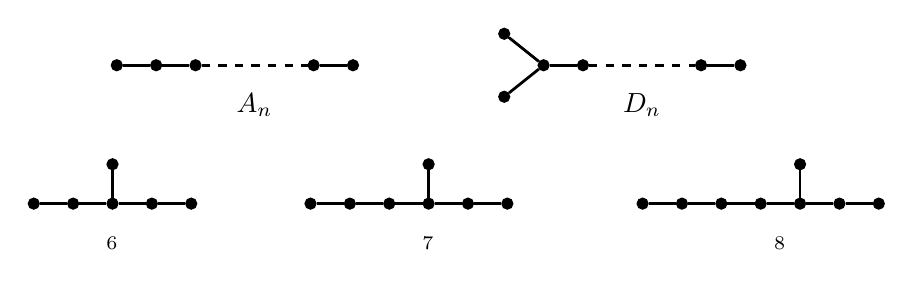
\begin{tikzpicture}
		\tikzset{dynode/.style={circle, draw, fill=black,
					minimum size=4pt, inner sep=0pt}}
		\tikzset{dyline/.style={line width=1pt}}
		\tikzset{dydash/.style={line width=1pt, dashed}}

		\begin{scope}[yshift=0, xshift=22em]
			\node[dynode] (a1) at (0,0) {};
			\node[dynode] (a2) at (0.5,0) {};
			\node[dynode] (a3) at (1,0) {};
			\node[dynode] (a4) at (1.5,0) {};
			\node[dynode] (a5) at (2,0) {};
			\node[dynode] (a6) at (2.5,0) {};
			\node[dynode] (a7) at (3,0) {};
			\node[dynode] (a8) at (2,0.5) {};

			\draw[dyline] (a1) -- (a2) -- (a3) -- (a4) -- (a5) -- (a6) -- (a7);
			\draw[dyline] (a5) -- (a8);

			\node[] (l) at (1.75,-0.5) {$\E_8$};
		\end{scope}

		\begin{scope}[yshift=0, xshift=10em]
			\node[dynode] (a1) at (0,0) {};
			\node[dynode] (a2) at (0.5,0) {};
			\node[dynode] (a3) at (1,0) {};
			\node[dynode] (a4) at (1.5,0) {};
			\node[dynode] (a5) at (2,0) {};
			\node[dynode] (a6) at (2.5,0) {};
			\node[dynode] (a8) at (1.5,0.5) {};

			\draw[dyline] (a1) -- (a2) -- (a3) -- (a4) -- (a5) -- (a6);
			\draw[dyline] (a4) -- (a8);

			\node[] (l) at (1.5,-0.5) {$\E_7$};
		\end{scope}

		\begin{scope}[yshift=0, xshift=0]
			\node[dynode] (a1) at (0,0) {};
			\node[dynode] (a2) at (0.5,0) {};
			\node[dynode] (a3) at (1,0) {};
			\node[dynode] (a4) at (1.5,0) {};
			\node[dynode] (a5) at (2,0) {};
			\node[dynode] (a8) at (1,0.5) {};

			\draw[dyline] (a1) -- (a2) -- (a3) -- (a4) -- (a5);
			\draw[dyline] (a3) -- (a8);

			\node[] (l) at (1,-0.5) {$\E_6$};
		\end{scope}

		\begin{scope}[yshift=5em, xshift=3em]
			\node[dynode] (a1) at (0,0) {};
			\node[dynode] (a3) at (0.5,0) {};
			\node[dynode] (a4) at (1,0) {};
			\node[dynode] (a5) at (2.5,0) {};
			\node[dynode] (a6) at (3.0,0) {};

			\draw[dyline] (a1) -- (a3) -- (a4);
			\draw[dydash] (a4) -- (a5);
			\draw[dyline] (a5) -- (a6);

			\node[] (l) at (1.75,-0.5) {$\op{A}_n$};
		\end{scope}

		\begin{scope}[yshift=5em, xshift=17em]
			\node[dynode] (a1) at (0,0.4) {};
			\node[dynode] (a2) at (0,-0.4) {};
			\node[dynode] (a3) at (0.5,0) {};
			\node[dynode] (a4) at (1,0) {};
			\node[dynode] (a5) at (2.5,0) {};
			\node[dynode] (a6) at (3.0,0) {};

			\draw[dyline] (a1) -- (a3);
			\draw[dyline] (a2) -- (a3);
			\draw[dyline] (a3) -- (a4);
			\draw[dydash] (a4) -- (a5);
			\draw[dyline] (a5) -- (a6);

			\node[] (l) at (1.75,-0.5) {$\op{D}_n$};
		\end{scope}
	\end{tikzpicture}
	\vspace{1em}
	\caption{\todo{describe}}
\end{figure}

Given a tree $T$ with weights $w$ in $\pi_{m-1}(\SO_m)$, we can form a manifold with boundary constructed in the following manner:
\begin{enumerate}
	\item For each vertex $v\in \op{Vert}(T)$, choose an $n$-disc bundle $\xi_v\to S^m_v$ classified by $w(v)\in \pi_{m-1}(\SO_m)$.
	\item For each edge $(v,w)\in \op{Edge}(T)$ connecting vertices $v$ and $w$, plumb together the bundles $\xi_v$ and $\xi_w$. For this to be well-defined, it's important to choose disjoint disc embeddings $\iota_{v,w} : D^m \to S^m_v$ for all $w$ connected to $v$.
	\item Smooth out the corners of the resulting space to get a manifold with boundary.
\end{enumerate}
\begin{definition}
	The \defn{plumbing} along the weighted tree $(T,w)$, denoted by $P(T,w)$ is the manifold with boundary described above.
\end{definition}

\begin{theorem}
	The result of this plumbing construction is independent of the choices of disc bundles $\xi_v$ and disc embeddings $\iota_{v,w} : D^m \to S^m_v$.
\end{theorem}

\begin{proof}
\end{proof}

\begin{remark}
	\todo{plumbing has a 1-skeleton homotopic to the tree}
\end{remark}

\begin{definition}\label{defn:E8-matrix}
\end{definition}

\subsection{Plumbing Constructions of 3-Manifolds}

\section{Knots and Complex Singularities}

Let $F\in \C[z_0,z_1\ldots, z_n]$ be a non-constant polynomial in $(n+1)$-complex variables.
\begin{definition}
	The \defn{variety} of $F$ is the complex hypersurface given by the zero locus
	\[
		\V(F) = F^{-1}(0)=\left\{ z \in \C^{n+1} \mid F(z)=0\right\} \subset \C^{n+1}.
	\]
\end{definition}

\todo{cauchy riemann equations}

\begin{definition}
	The \defn{gradient} of a complex analytic function $F : \C^{n+1} \to \C$ is the $(n+1)$-tuple
	\[
		\nabla_F = \left(\frac{\partial F}{\partial z_0}, \frac{\partial F}{\partial z_1},\ldots, \frac{\partial F}{\partial z_n}\right).
	\]
	\todo{better definition}
\end{definition}

\begin{definition}
	A point $w\in \V(F)$ is a (complex) \defn{singularity}[complex singularity] if $\nabla_F(w)$ vanishes. A singularity is \defn{isolated}[isolated singularity] if there is a neighborhood surrounding $w$ which contains no other singularities.
\end{definition}

\begin{theorem}
  For small $\varepsilon>0$ the intersection of $\V(F)$ with $D_\varepsilon(w)$
\end{theorem}

\begin{proposition}
	Every sufficiently small sphere around an isolated singularity of $F$ intersects $\V(F)$ transversally in a smooth manifold.
\end{proposition}

\begin{definition}
	Let $w\in \V(F)$ be an isolated singularity. The \defn{link} of $F$ at $w$ is the intersection
	\[
		\L(F, w) = \V(F) \cap S^{2n+1}_\varepsilon(w) = \left\{ z\in \C^{n+1} \mid F(z)=0\textrm{ and } |z-w|<\varepsilon\right\}
	\]
	where $\varepsilon > 0$ is some sufficiently small real number so that $\L(F,w)$ is a smooth manifold intersecting the sphere $S^{2n+1}_\varepsilon(w)$ transversally.
\end{definition}

When the isolated singularity is clear, we write $\L(F)$.

\subsection{Brieskorn Manifolds}
The simplest examples of complex polynomials with isolated singularities are \todo{this}

\begin{definition}
	Let $(a_0,a_1,\ldots, a_n)$ be an $(n+1)$-tuple of integers greater than or equal to $2$. The \defn{Brieskorn polynomial} of the tuple $(a_0,a_1,\ldots, a_n)$ is given by
	\[
		F(z_0,z_1,\ldots, z_n) = z_0^{a_0} + z_1^{a_1} +\cdots + z_n^{a_n}.
	\]
	Correspondingly, we refer to $\V(F)$ as the \defn{Brieskorn variety} of the tuple and to the link at the origin $\L(F,0)$ origin as the \defn{Brieskorn manifold}. We'll use the notation
	\[
		\Sigma(a_0,a_1,\ldots, a_n) =\L(z_0^{a_0}+z_1^{a_1}+\cdots+z_n^{a_n}, 0)
	\]
	to refer to these Brieskorn manifolds.
\end{definition}


\begin{proposition}
	If $p,q\geq 2$, then $\Sigma(p,q)\subset S^3$ is the torus link of type $(p,q)$.
\end{proposition}

\begin{proposition}
	There is a homeomorphism $\Sigma(2,2,2)\cong \RP^3$.
\end{proposition}

\begin{proposition}
	There is a homeomorphism $\Sigma(2,3,5)\cong \mathscr{D}$.
\end{proposition}

\subsection{The Fibration Theorem}

\begin{theorem}\label{thm:fibration}
	If $F$ is a complex polynomial in $(n+1)$-variables with an isolated singularity at the origin, then there is a smooth fiber bundle map
	\[
		\lkxfunc{\phi}{S^{2n+1}_\varepsilon - \L(F)}{S^1}{z}{\arg F(z).}
	\]
\end{theorem}

For a given angle $e^{i\theta}\in S^1$, we'll denote the fiber of the bundle $\phi$ as $F_\theta = \phi^{-1}(e^{i\theta})$.

\begin{proposition}
  Each fiber $F_\theta$ is a smooth parallelizable $2n$-manifold.
\end{proposition}

\subsection{When is the link a topological sphere?}

Let's fix a polynomial $F$ in $(n+1)$ complex variables

\begin{proposition}
  If $n\neq 2$, then $\L$ is homeomorphic to the sphere $S^{2n-1}$ if and only if $\L$ has the homology of a sphere. In fact, $\L$ is a topological sphere if and only if the reduced homology $\widetilde{H}_{n-1}(\L)$ is trivial.
\end{proposition}

Let's now choose an orientation for $F_\theta$.

\begin{proposition}
  The manifold $\L$ is a homology sphere if and only if the intersection form
  \[
    \lkxfunc{Q_{F_\theta}}{\H_n(F_\theta)\times \H_n(F_\theta)}{\Z}
  \]
  has determinant $\pm 1$ -- in other words if $Q_{F_\theta}$ is unimodular.
\end{proposition}

\section{Kervaire Invariant}

\begin{theorem}[Brieskorn-Pham]
\end{theorem}

\begin{theorem}[Levine]
  If $n$ is odd, the Kervaire invariant is given by
  \[
    c(F_0) = \begin{cases} 
      0 & \textrm{if }\Delta(-1)\equiv \pm 1\mod 8\\
      1 & \textrm{if }\Delta(-1)\equiv \pm 3\mod 8
    \end{cases}
  \]
\end{theorem}

\begin{theorem}[Hirzebruch-Mayer] Smooth Brieskorn varieties are parallelizable.
\end{theorem}
